\startchapter{Quantitative Analysis}
\label{chapter:quantAnalysis}
\section{Introduction}
Samer Moein originally proposed a series of techniques for the express purpose of quantifying the hardware security science in his Ph.D dissertation \textit{Systematic Analysis and Methodologies for Hardware Security} \cite{SamerDissertation}. This chapter will provide an overview of these techniques which are the basis for the \textit{Hardware Trojan System}.
\section{Classification} \label{section:Classification}
To properly understand the wide-ranging forms and origins of trojans a classification system is used that employs their key aspects \cite{SamerDissertation}, \cite{SamerClassification}. A list of thirty-three attributes is proposed that quantify the characteristics of hardware trojans. Each of the attributes are taxonomically grouped into one of eight classes as outlined in Figure~\ref{fig:HW_trojan}. These taxonomic classes are then further organized into the four main categories as shown in Figure~\ref{fig:trojan_life_cycle} that are used by the classification tool discussed later in section ~\ref{Application:Classification}. These four primary categories are:

\begin{enumerate}
	\item The \textbf{Insertion} category (also know as the \textit{Chip Life Cycle} category) comprises attributes pertaining to the stages of production of an IC that are vulnerable to malicious attack.
	\item The \textbf{Abstraction} category looks at the abstraction level of the IC in which a trojan is introduced.
	\item The \textbf{Properties} section is comprised of qualities all pertaining to the observed behaviors and physical construction of trojans. This main category is the only one of the four that contains more than one of the taxonomic classes: \textit{effect}, \textit{logic type}, \textit{functionality}, \textit{abstraction} and \textit{layout}. 
	\item The \textbf{Location} category looks at the physical place in the integrated circuit where the trojan lies.
\end{enumerate}
\begin{figure}
	\centering
	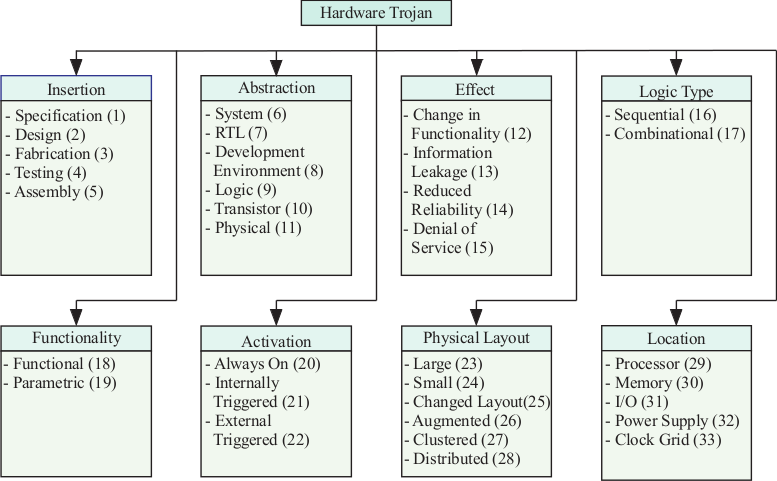
\includegraphics[width=0.95\linewidth]{figures/HW_trojan}
	\caption[The Taxonomy of Attributes and Subcategories]{The Taxonomy of Attributes and Subcategories}
	\label{fig:HW_trojan}
\end{figure}
\begin{figure}
	\centering
	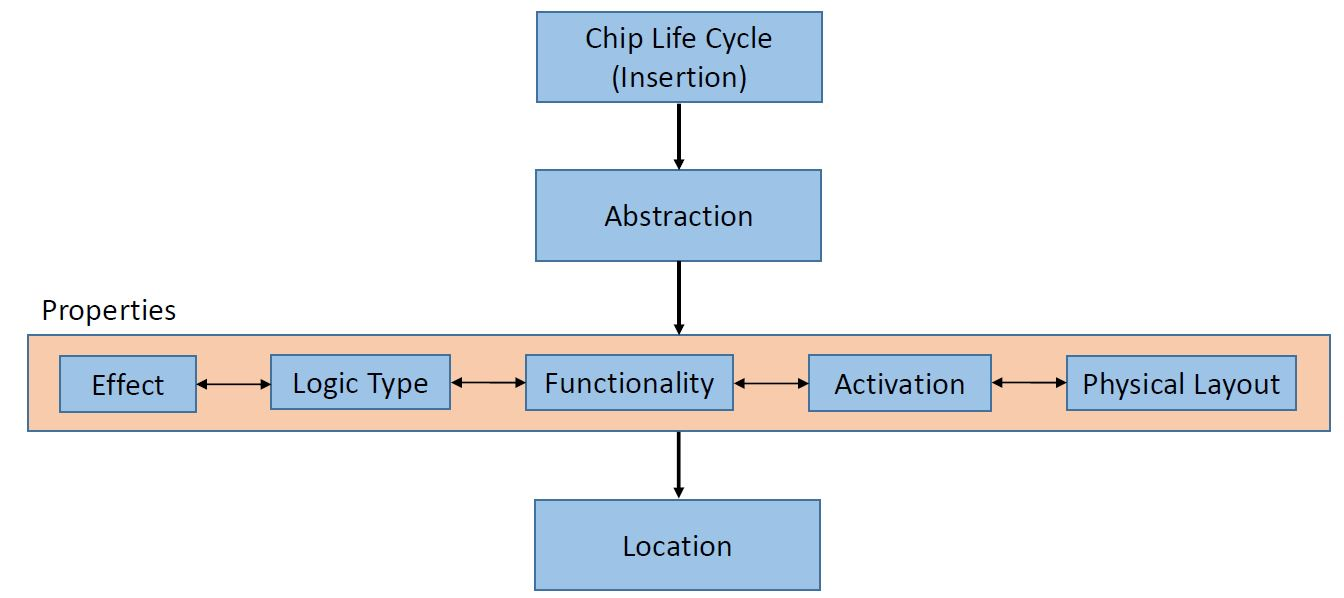
\includegraphics[width=0.7\linewidth]{figures/trojan_life_cycle}
	\caption[Hardware Trojan Levels of the Four Main Categories]{Hardware Trojan Levels of the Four Main Categories}
	\label{fig:trojan_life_cycle}
\end{figure}

When a trojan is discovered it is analyzed for the possession of the attributes from the \textit{Properties} category. An $n$x$n$ relation matrix, referred to as $R$, is used to relate each of the thirty-three attributes to each and every other attribute. Due to its size the matrix $R$ is not included in this paper however it is summarized in Figure~\ref{fig:R_short}; refer to \cite{SamerClassification} for the whole matrix $R$. Each entry in the matrix, denoted $r(i,j)$, represents whether attribute $i$ can lead to attribute $j$. For example, referring to Figure~\ref{fig:R1}, an entry $r(2,3) = 1$ indicates that attribute 2 \textit{(Design)} can lead to attribute 3 \textit{(Fabrication)}. Colloquially this means that if a malicious member of the design team is capable of compromising the integrated circuit during the design phase (insertion point 2) the damage can propagate to the fabrication phase (insertion point 3). 

\begin{figure}
	\centering
	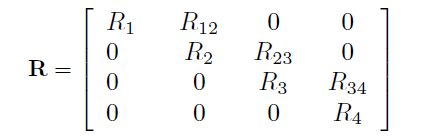
\includegraphics[width=0.5\linewidth, scale=0.5]{figures/R_short}
	\caption[Matrix R. Sub matrices Composition]{Matrix R. Sub matrices Composition}
	\label{fig:R_short}
\end{figure}

This relationship between attribute two and three can be described as \textit{"inter-category"} as both the source and target attributes belong to the same category, \textit{insertion}. Non \textit{"inter-category"} relationships relate attributes of different categories. For example, from the \textit{Abstraction} category, a virus that is introduced in the \textit{Register Transfer Level} (attribute 7) can not directly cause a trojan that exhibits the \textit{Reduced Reliability} (attribute 14) property because the relation $r(7,14) = 0$. The same virus is however capable of causing a \textit{Denial of Service} because the relation $r(7,15) = 1$.

The matrix R is divided into sub matrices as shown in Figure~\ref{fig:R_short}. Sub matrices $R_{1}$, $R_{2}$, $R_{3}$ and $R_{4}$ contain the \textit{"inter-category"} relations; sub matrix $R_{1}$ is show in detail in Figure~\ref{fig:R1}. Notice how the same attributes (1-5) are represented in both the rows and columns. 

\begin{figure}[h]
	\centering
	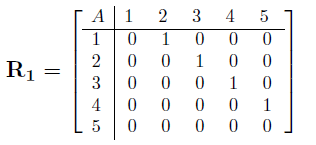
\includegraphics[width=0.45\linewidth]{figures/R1}
	\caption[Sub Matrix R1, \textit{"inter-category"} Example]{Sub Matrix R1, \textit{"inter-category"} Example}
	\label{fig:R1}
\end{figure}

Non \textit{"inter-category"} sub matrices provide the relations of attributes from one category to another. Figure~\ref{fig:R12} shows an example of a non \textit{"inter-category"} sub matrix. $R_{12}$ relates the insertion point attributes of matrix $R_{1}$ to the abstraction level attributes of $R_{2}$. Suppose it is found that a trojan pertains only to the abstraction \textit{"Register Transfer Level"} (attribute number 7). Inspection of column 7 in Figure~\ref{fig:R12} determines that the only possible insertion point is attribute number 2 (Design). This tells us that the only part of the production life cycle where a malicious person could have inserted this virus was during the design phase. This method has drastically reduced the search time for the guilty party.

\begin{figure}
	\centering
	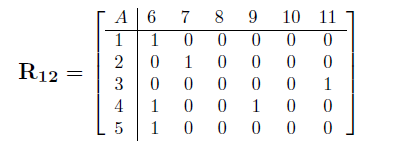
\includegraphics[width=0.5\linewidth]{figures/R12}
	\caption[Sub Matrix R12, non \textit{"inter-category"} Example]{Sub Matrix R12, non \textit{"inter-category"} Example}
	\label{fig:R12}
\end{figure}

Matrix $R$ allows us to visualize the nature of the trojan via a directed graph. Figure~\ref{fig:Full1} shows an example visualization of a virus that was discovered to have properties $12$, $17$, $18$, $21$, $24$, $26$ and $27$. For a more detailed explanation of how each of the attributes relate and how the matrix $R$ is used to analyze a trojan please refer to \cite{SamerDissertation} and \cite{SamerClassification}.
\begin{figure}[h]
	\centering
	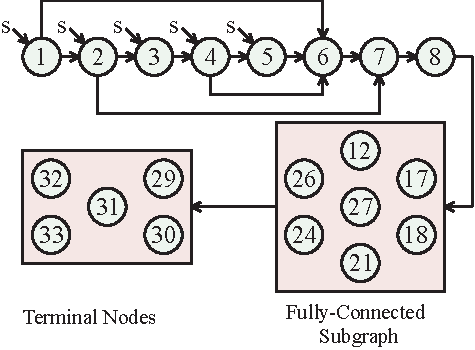
\includegraphics[width=0.55\linewidth]{figures/Full1}
	\caption[Directed Graph of Example Virus]{Directed Graph of Example Virus}
	\label{fig:Full1}
\end{figure}

\section{Detection} \label{section:Detection}
The lack of consistent structure across the spectrum of processor design results in a massive diversity in regards to the structure, behavior and insertion points of trojans and as of yet there is no single method of detection capable of handling all possibilities. Specific trojan characteristics requires equally specific means of detection. The natural segregation of each individual trojan detection pair makes it extremely difficult to compare and contrast competing techniques. To combat such ambiguity a ranking system has been developed that will not only aid in the selection and definition of detection methods but will aid in the selection of techniques based on observed characteristics of trojans.\newline

To construct a means of comparison between a trojan and a detection scheme each are given a numerical value representing the level of applicability in each of the eight classes outlined in Figure~\ref{fig:HW_trojan}. When a trojan virus is analyzed using the classification method described in section \ref{section:Classification} the selected attributes are used to create a series of values to build a vector known as the trojan's \textit{Severity} ranking. Each class contains multiple attributes, the combination of the attributes present in a trojan are the determining factor for the assigned value. Figure~\ref{fig:effectSeverity} shows the ranking table for the \textit{effect} class. Every class is assigned two values, one to represent the unique combination ($I_E$ in this class) and a second to represent the severity level ($C_E$). \newline

\begin{figure}[h]
	\centering
	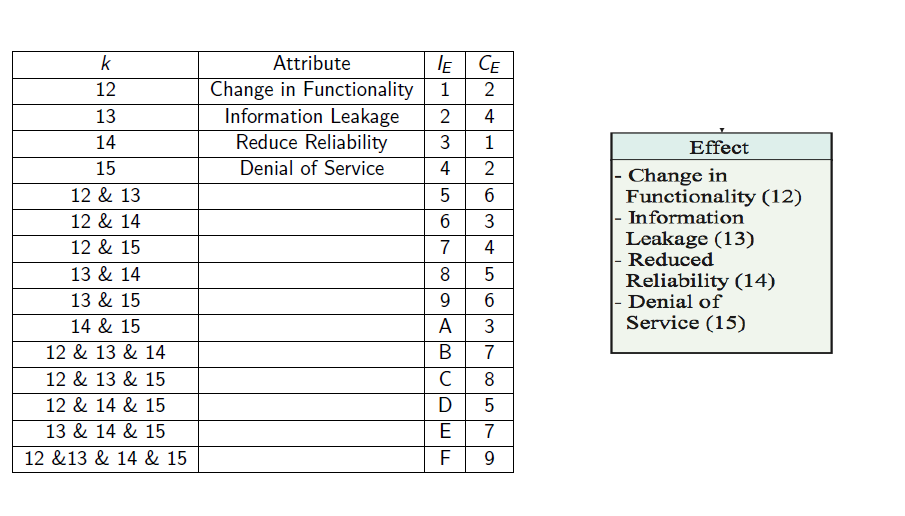
\includegraphics[width=0.8\linewidth]{figures/effectSeverity}
	\caption[The Ranking Values of The Effect Class]{The Ranking Values of The Effect Class}
	\label{fig:effectSeverity}
\end{figure}

Table~\ref{tbl:severityTable} provides an example of the use of the severity rating of two hardware trojans. With use of this ranking system two completely different viruses can be quantitatively compared and contrasted for efficacy in each class. When a new detection method is produced the same ranking tables are used to produce a similar vector where the only difference is that the severity value is referred to as the method's \textit{Coverage Level}. Coverage is used to determine the methods ability to detect a trojan of a common class. Table~\ref{tbl:detectionTable} shows the coverage vectors of two detection methods. By comparing these methods with the trojans in Table~\ref{tbl:severityTable} a user can quickly and accurately determine the applicability of a method for a particular trojan. By comparing \textit{Trojan A} with detection method $6$ it can be seen that the insertion point ranking value ($I_R$) is higher in the detection method than it is in the trojan. This implies that method $6$ would be an appropriate choice for detecting \textit{Trojan A} in regards to where it is inserted. For a complete description of the ranking tables and more thorough discussion of their application refer to \cite{SamerDetection}.\newline

\begin{table}[h]
	\centering
	\caption{Severity Rating Vectors of two Trojans}
	\label{tbl:severityTable}
	\renewcommand{\arraystretch}{1.2}
	\begin{tabular}{|c|p{0.3mm}p{0.3mm}p{0.3mm}p{0.3mm}p{0.3mm}p{0.3mm}p{0.3mm}p{2mm}|p{0.3mm}p{0.3mm}p{0.3mm}p{0.3mm}p{0.3mm}p{0.3mm}p{0.3mm}p{2mm}|}
		\hline
		Techniques & \multicolumn{8}{c|}{Parameters ($I_P$)} & \multicolumn{8}{c|}{Severity ($C_P$)} \\ \cline{2-17} 
		& $I_R$ & $I_A$ & $I_E$ & $I_L$ & $I_F$ & $I_C$ & $I_P$ & $I_O$ & $C_R$ & $C_A$ & $C_E$ & $C_L$ & $C_F$ & $C_C$ & $C_P$ & $C_O$ \\ \hline
		Trojan A & 2 & 6 & 2 & 1 & 2 & 1 & 7 & 7 & 2 & 6 & 4 & 1 & 2 & 1 & 5 & 2 \\ \cline{1-1}
		Trojan B & 3 & 3 & 1 & 2 & 1 & 2 & 8 & 1 & 3 & 3 & 2 & 2 & 1 & 3 & 6 & 1 \\ \hline
	\end{tabular}
\end{table}
\begin{table}[h]
	\centering
	\caption{Hardware Trojan Detection Vector}
	\label{tbl:detectionTable}
	\renewcommand{\arraystretch}{1.2}
	\begin{tabular}{|c|p{1mm}p{1mm}p{1mm}p{1mm}p{1mm}p{1mm}p{1mm}p{1mm}p{2mm}|p{1mm}p{1mm}p{1mm}p{1mm}p{1mm}p{1mm}p{1mm}p{1mm}p{2.5mm}|}
		\hline
		Techniques & \multicolumn{9}{c|}{Parameters ($I_P$)} & \multicolumn{9}{c|}{Coverage ($C_P$)} \\ \cline{2-19} 
		& $I_R$ & $I_A$ & $I_E$ & $I_L$ & $I_F$ & $I_C$ & $I_P$ & $I_O$ & $I_G$ & $C_R$ & $C_A$ & $C_E$ & $C_L$ & $C_F$ & $C_C$ & $C_P$ & $C_O$ & $C_G$ \\ \hline
		\cite{detectionMethod1} & 3 & 3 & B & 1 & 2 & 4 & 7 & V & 1 & 3 & 3 & 7 & 1 & 2 & 3 & 5 & 5 & 2 \\ \cline{1-1}
		\cite{detectionMethod2} & 3 & 3 & 1 & 2 & 1 & 4 & 7 & V & 4 & 3 & 3 & 2 & 3 & 1 & 3 & 5 & 5 & 3 \\ \hline
	\end{tabular}
\end{table}

Table~\ref{tbl:severityTable} gives a side by side comparison of the severity rating vectors for two trojan viruses. Trojan \textit{A} has a lower coverage rating value than Trojan \textit{B} in the \textit{Insertion} subcategory denoted by $C_R$. This signifies that Trojan B could be inserted in more stages of the manufacture process than Trojan \textit{A} making it a more dangerous virus. Table~\ref{tbl:detectionTable} gives a similar comparison between two competing detection methods. Method 6 has a higher coverage rating in the \textit{effect} subcategory than method 16 signifying there is a larger number of virus effects this method is able to detect. By referring to Table~\ref{tbl:detectionTable} and Figure~\ref{fig:effectSeverity} it can be devised that method 6 is capable of detecting attributes $12$, $13$ and $14$ where as method 16 is only capable of detecting attribute $12$. Further more it is possible to compare a virus and a detection method in a similar manner. In this scenario the special case of the virus and method having an equal coverage/severity rating the detection method's coverage rating value takes precedence over the virus's severity. Colloquially this implies that a coverage rating is capable of detecting a severity rating of an equal value.

\section{Attacks} \label{section:Attacks}

